%\documentclass[a4paper,twoside,11pt]{report}
\documentclass[a4paper,singleside,11pt]{report}

\usepackage{ia_urb_thesis}
\usepackage[italian]{babel}
\usepackage[latin1]{inputenc}
\usepackage[T1]{fontenc}
\usepackage{lmodern}
\usepackage{amsmath,
	    amsfonts,
	    amstext,
	    amssymb,
	    mathrsfs,
	    stmaryrd,
	    latexsym,
	    %enumitem,
	    proof,
	    graphicx,
	    epsfig,
	    color,
	    %hyperref,
	    comment}

\begin{document}

\titolo{Cos'\`e Blazor?}
\candidato{Francesco Belacca}
\relatore{Chiar.mo Prof.~Emanuele Lattanzi}
\annoaccademico{2018-2019}

\copertinatesi 
\dedica{A tutti quelli che mi hanno detto almeno una volta di non mollare.}
\indice
\indicefigure
%\indicetabelle
\iniziatesto

\chapter{Introduzione}\label{cap:introduzione}

\section{Contesto}\label{sez:contesto}

A seguito della crescita esponenziale del web in questo secolo e dell'abituarsi di tutti coloro che ne usufruiscono ad un livello grafico sempre migliore e ad una esperienza mano a mano pi\`u interattiva e vicina all'utente medio, i siti web e le tecnologie utilizzate si sono adattati per permettere uno sviluppo sempre pi\`u rapido di codice pi\`u facilmente testabile e mantenibile.

Di conseguenza nel frontend si sono susseguiti una serie di framework e di strumenti, a partire da JQuery\cite{jquery} nel 2006, che per primo si \`e occupato di risolvere il problema della compatibilit\`a tra browsers, permettendo ai developers di scrivere una volta, e poter eseguire su tutti i browsers.

AngularJS nel 2010 \`e stato il primo MVC framework ad offrire in un unico pacchetto un insieme di features che hanno facilitato tantissimo la vita ai developers, come il two-way data binding, la dependency injection, il routin, oltre ad altri strumenti utili per rendere pi\`u standard lo sviluppo nel frontend~\cite{Hoff}.
Questo framework largamente utilizzato, \'e stato riscritto nel 2013 diventando Angular 2 (e nelle versioni pi\'u recenti rinominato semplicemente in Angular) senza mantenere retrocompatibilit\`a e senza offrire un modo preciso per migrare alla nuova versione agli utilizzatori di AngularJS.
Anche per questo React, un nuovo framework pi\`u leggero e modulare sviluppato dagli sviluppatori di Facebook, ha preso il posto di Angular come framework pi\`u utilizzato nel frontend.

Vue infine \'e il terzo dei principali framework che ha provato a prendere piede proponendo una versione intermedia tra il fortemente opinionato Angular e il pi\'u flessibile React.

Oltre a questi, ciascuno con la propria semantica, organizzazione logica dei folder, spesso una CLI dedicata, ad un developer frontend viene solitamente richiesto di conoscere HTML, CSS e chiaramente Javascript essendo ci\'o su cui si basano poi i vari framework.

Oltre a Javascript, se si vuole scrivere degli unit test facilmente mantenibili, bisogna conoscere TypeScript(specialmente se si utilizza Angular, che rende il suo utilizzo obbligatorio) e degli altri framework che facilitino i test(Enzyme, Karma + Jasmine, ...).

\section{Problema}\label{sez:problema}
I continui cambiamenti nei molti framework utilizzati, la diversit\`a degli strumenti stessi tra loro, che spesso realizzano in modo diverso tutti la stessa cosa, rendono sempre pi\'u difficile per un junior developer iniziare a sviluppare, vista l'ampia curva di apprendimento e lo studio necessario, per poter essere spendibile a livello professionale.

Oltretutto un web developer ad oggi finisce per essere costretto a scegliere se diventare uno sviluppatore frontend o backend, dato che rimanere al passo e aggiornarsi gi\`a in solo uno di questi due campi richiede tempo e non \`e scontato ad esempio che venga concesso di poterlo fare in orario lavorativo, pur essendo fondamentale.

\'E quindi chiaro che per tutti i web developer, e specialmente per una figura mista spesso identificata con il titolo "Full-Stack Developer", ci sia una continua ricerca del modo per rendere le proprie competenze quanto pi\'u trasversali possibile, anche in termini di tecnologia utilizzata.

\pagebreak

\section{Linguaggi General-Purpose}\label{sez:problema}
Microsoft, nel backend e in ambito applicativo, ha reso nel tempo il framework .NET e le sue implementazioni(.NET Core, .NET Framework e Mono) utilizzabili nei vari propri linguaggi, C\#, F\# e VB.
La figura 1.1 qui di seguito riassume le implementazioni del .NET Standard e le varie tipologie di applicazioni che si possono sviluppare con ciascuna.

\begin{figure}[H]
	\centerline{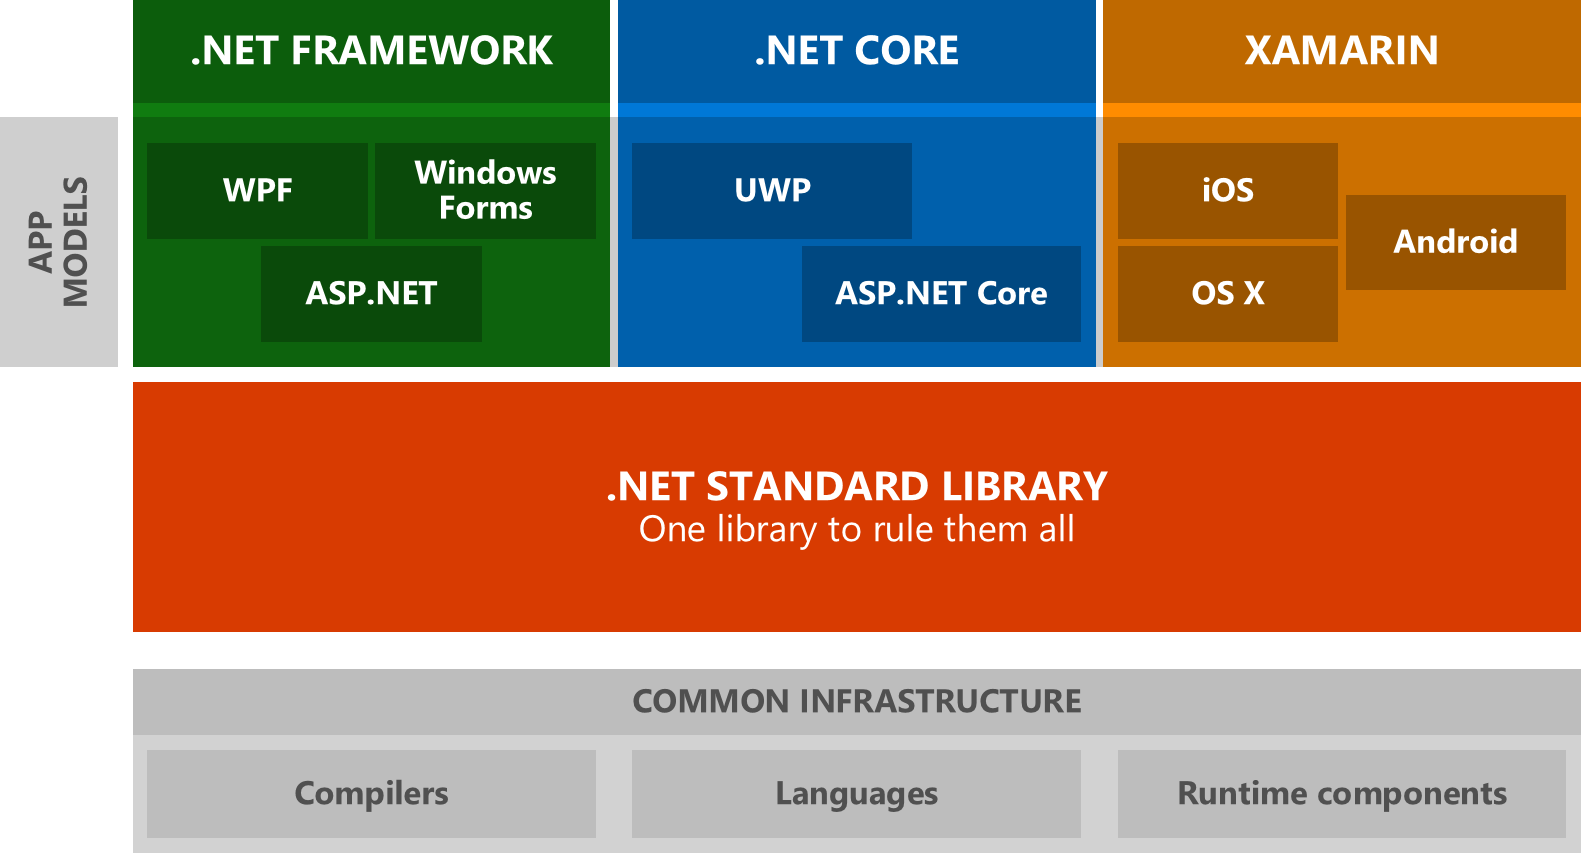
\includegraphics[scale=0.2]{figure/DotNetImplementations}}
	\caption{Implementazioni del .NET Standard}
	\label{fig:DotNetImplementations}
\end{figure}

Scrivendo ad esempio in C\# \`e possibile sviluppare vari tipi di applicazioni come si pu\'o vedere nella figura 1.2, ma se si decide di sviluppare codice per un applicazione client web ad oggi si \`e ancora costretti a scrivere utilizzando Javascript e un suo framework se si vuole essere veloci nello sviluppo e scrivere codice mantenibile specialmente in team pi\'u grandi, come nel mondo enterprise.

\begin{figure}[H]
\centerline{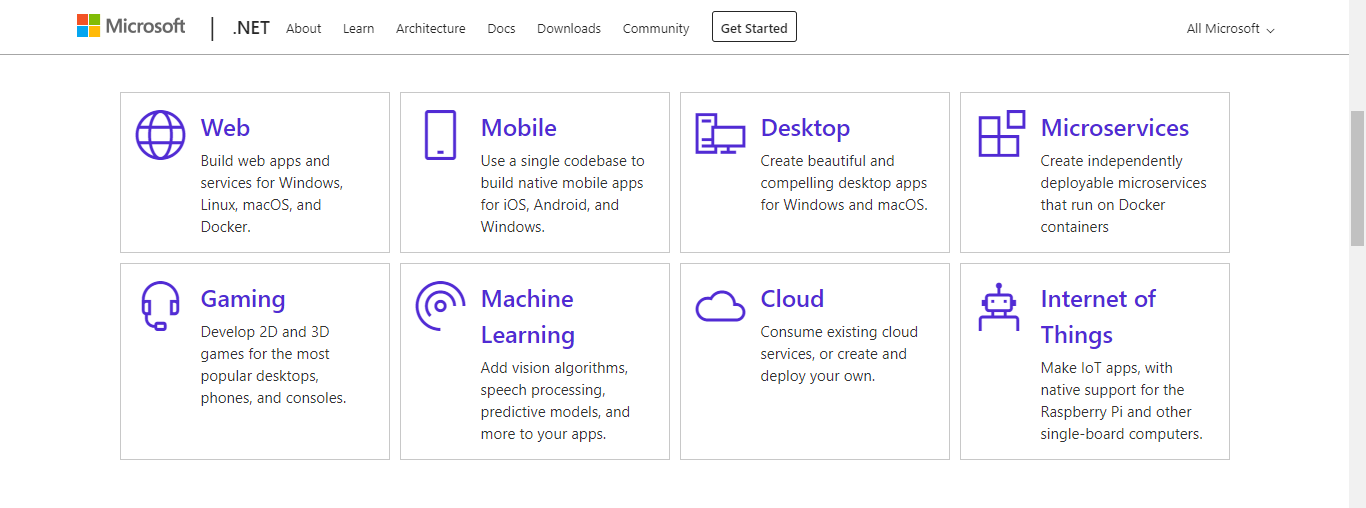
\includegraphics[scale=0.35]{figure/DotNetFrameworkCapabilities}}
\caption{Possibilit\'a di .NET}
\label{fig:DotNetCapabilities}
\end{figure}

Gi\'a con Razor\cite{razor}, Microsoft ha permesso la generazione di codice HTML e CSS in modo dinamico utilizzando C\#, ma \`e utilizzabile solo lato server e quindi la cattura di un evento client side come il click di un utente su un bottone, senza contattare il server, non \`e stato possibile fino ad ora senza passare per Javascript.

\section{Blazor}
Ecco cosa \'e quindi Blazor: la versione pi\'u avanzata di Razor(Browser+Razor\cite{blazorWikiGitHub}) che permette ai developer di gestire anche gli eventi client-side, direttamente in C\#(o nel linguaggio scelto tra quelli supportati) come se questo fosse effettivamente ci\'o che viene eseguito lato client, mentre in reat\'a l'esecuzione lato client cambia a seconda del modello scelto, come poi vedremo pi\'u nel dettaglio.

Blazor utilizza per i vari modelli, delle tecnologie diverse(ad esempio il WebAssembly) ma che rispettano sempre lo standard del web.
Non \'e invece un plugin da installare, e non dipende da un browser specifico.
Non \'e nemmeno una "semplice" tecnologia di transpilazione verso javascript, contrariamente a tecnologie come TypeScript.
\chapter{Modelli e Funzionamento}\label{cap:modefunz}
\section{Blazor Server}\label{sez:bserver}
Il primo dei modelli ufficialmente rilasciati e per il quale si pu\'o ricevere supporto in produzione da settembre 2019\cite{blazorServerRelease}, \'e proprio questo.

Un'applicazione Blazor Server ospita i componenti Blazor lato Server e gestisce le interazioni dell'utente con la UI attraverso una connessione in tempo reale sfruttando SignalR, come visibile nella figura 2.1.

\begin{figure}[H]
	\centerline{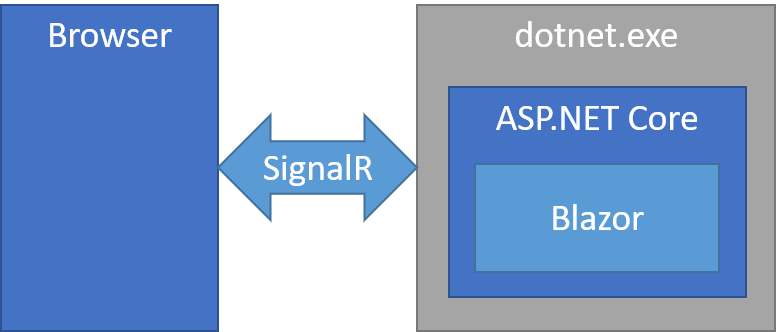
\includegraphics[scale=0.6]{figure/blazor-server.png}}
	\caption{Blazor Server}
	\label{fig:BlazorServer}
\end{figure}

Ci\'o significa che quando un utente scatena un evento, questo viene inviato attraverso la real time connection al server, dove il rispettivo componente di competenza gestisce l'evento.
Quando l'evento \'e stato gestito, blazor compara l'output appena generato con quello precedente all'evento, e manda quindi le sole differenze al browser del client, per poi applicarle al DOM.\cite{blazorModelsScenarios}

Blazor Server perci\'o necessita di una connessione stabile e a bassa latenza per funzionare al meglio, e gli scenari offline non sono supportati.
Ci\'o significa anche che la posizione del server sul quale \'e ospitata l'applicazione non pu\'o essere troppo distante dal client che si sta connettendo per garantire un funzionamento senza lag.

\'E particolarmente indicato quando si vuole delegare il costo computazionale al server e non ai client connessi, dato che ci\'o che il client esegue \'e il solo codice statico e le differenze di volta in volta inviate ma calcolate lato server.
Ci\'o rende molto veloce ed efficiente il download e l'avvio dell'applicazione lato client, il che lo rende il modello perfetto per funzionare su apparecchi a basso costo.

\subsection{BlazorPong }\label{sez:bpong}
Un'esempio di applicazione scritta con questo modello, \'e BlazorPong, da me implementata e la cui demo \'e disponibile sul relativo repository in GitHub\cite{blazorPong}.

\begin{figure}[H]
	\centerline{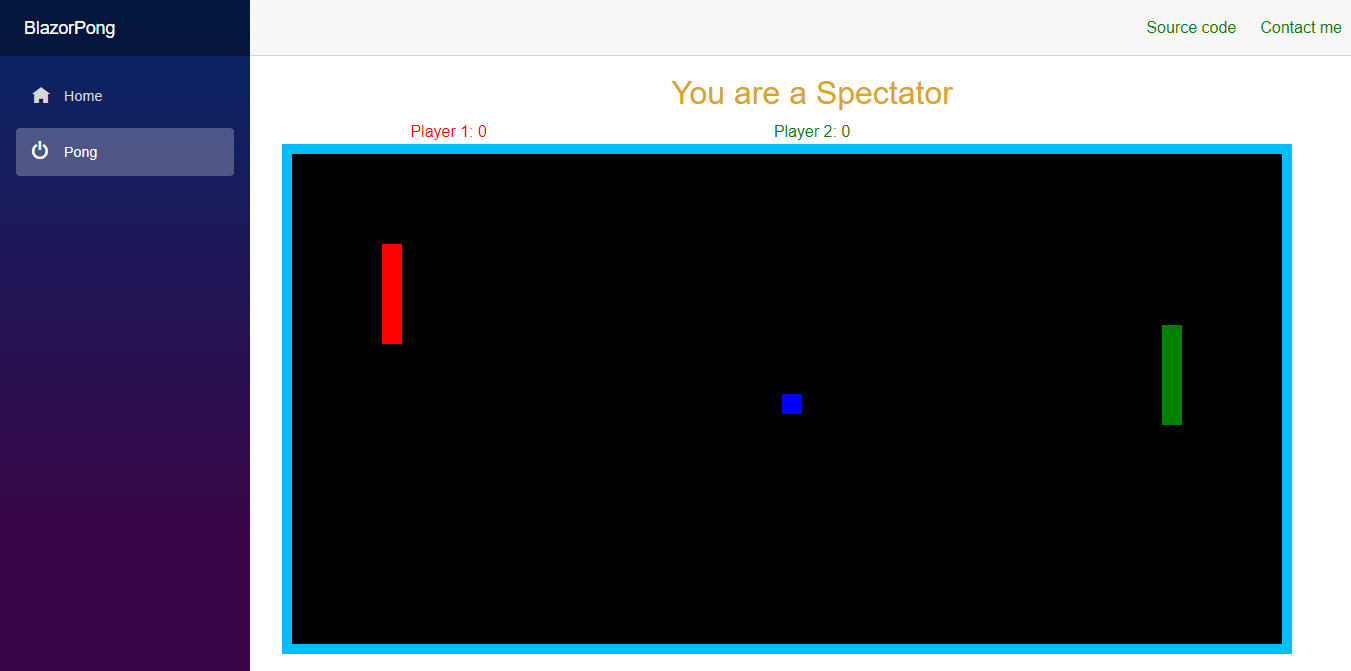
\includegraphics[scale=0.3]{figure/BlazorPong.PNG}}
	\caption{BlazorPong}
	\label{fig:BlazorPong}
\end{figure}

Visibile nella figura  questa applicazione permette a due giocatori che si collegano al sito contemporaneamente di giocare, e ai successivi utenti che si collegano di visionare la partita in corso come spettatori in tempo reale.
In questa applicazione ho scelto di utilizzare il modello server side per vari motivi:
\begin{enumerate}
	\item Il service worker che si occupa di aggiornare la posizione della pallina su tutti i client connessi, deve essere eseguito in un unico thread utilizzato per tutti i client connessi al server, ad ognuno dei quali invece devono arrivare gli aggiornamenti.
	\item Il calcolo delle differenze da applicare a ciascun DOM di ciascun utente connesso, per quanto avvenga continuamente(60fps circa), conviene avvenga direttamente lato server poich\'e l'applicazione \'e molto semplice e infatti anche un host di livello gratuito come quello che ho utilizzato riesce a far giocare senza problemi due persone con diversi spettatori(i test che ho fatto sono tutti dall'europa, poich\'e il server utilizzato si trova in Francia).
	\item Essendo la gestione degli eventi server side, il gioco pu\'o essere visualizzato in modalit\'a spettatore senza problemi anche su cellulari non molto performanti.
	
\end{enumerate}

Il funzionamento \'e piuttosto semplice: una volta che l'applicazione \'e stata avviata e che ciascun player si \'e connesso al sito ed ha cliccato play, quindi quando entrambi gli utenti sono pronti a giocare, inizia la partita.
Lato server viene gestito lo spostamento costante della pallina ed eventuali collisioni con muri verticali, orizzontali o con il blocco di uno dei player.
Rispettivamente gli eventi gestiti direttamente dal background worker sono quindi:
\begin{enumerate}
	\item Punto per il player dal lato opposto in cui avviene la collisione con un muro verticale;
	\item Inversione della velocit\'a di spostamento della pallina sull'asse y a seguito di una collisione con un muro orizzontale;
	\item Inversione della velocit\'a di spostamento della pallina sugli assi x ed y a seguito di una collisione con uno dei player;
	\item Invio di messaggio di fine partita contenente il player vincitore a tutti gli utenti connessi quando un utente arriva a 3 punti o uno dei due player si disconnette.
\end{enumerate}

Ci\'o che invece avviene grazie all'utente, \'e lo spostamento del proprio player attraverso l'evento di drag del proprio blocco.
Ad ogni evento scatenato dall'utente, la connessione SignalR invia l'evento al server, che lo processa e restituisce a tutti gli utenti connessi(compreso quello che ha scatenato l'evento) la differenza di CSS necessaria a far combaciare la nuova posizione reale del blocco del player che si \'e mosso, con l'immagine visualizzata.

\pagebreak

\section{Blazor WebAssembly}\label{sez:bwa}
Blazor WebAssembly \'e un modello attualmente in preview, che verr\'a ufficialmente rilasciato nella prima parte del 2020.

In questo modello il codice della SPA viene eseguito completamente lato client come solitamente avviene quando si utilizza un framework moderno per UI basato su JS, come i gi\'a citati Angular,React,Vue.

\begin{figure}[H]
	\centerline{\includegraphics[scale=0.6]{figure/blazor-WebAssembly.png}}
	\caption{Blazor WebAssembly}
	\label{fig:BlazorWebAssembly}
\end{figure}

Vengono quindi scaricati dal client l'applicazione Blazor, le sue dipendenze, ed il runtime del .NET scelto come target per l'applicazione.
L'applicazione viene quindi eseguita direttamente nel thread della User Interface del Browser utilizzato, come visibile nella figura 2.2.

L'ambito di esecuzione \'e la stessa sandbox di qualsiasi altra applicazione scritta con javascript, ossia il browser che si sta utilizzando.
Ci\'o \'e importante perch\'e implica(ed \'e cos\'i) che una web app scritta utilizzando Blazor non pu\'o fare niente di pi\'u o di meno di una web app standard.
Ogni update alla UI e la relativa gestione, avvengono utilizzando lo stesso processo nel browser.
Per questo modello, blazor.WebAssembly.js \'e il nome dello script Javascript che si occupa di scaricare il .NET runtime, l'applicazione e le dipendenze, come anche dell'inizializzazione dell'applicazione.

\subsection{WebAssembly}\label{sez:webAssembly}
In particolare il nome Blazor WebAssembly \'e stato scelto perch\'e utilizzlato client il codice viene eseguito grazie al file mono.wasm, ossia la compilazione del Runtime del framework Mono in WebAssembly, e Mono \'e una delle implementazioni esistenti del framework di base .NET Standard.
Il WebAssembly, che \'e un open standard che definisce un formato portatile di codice binario per programmi eseguibili e il rispettivo linguaggio assembly, come anche delle interfacce per facilitare le interazioni del codice con il proprio host.
\'E anche detto il byte code del web, dato che dal 2017 i browser pi\'u diffusi al mondo si sono impegnati per svilupparlo ed adottarlo.\cite{webAssemblySupport}

\begin{figure}[H]
	\centerline{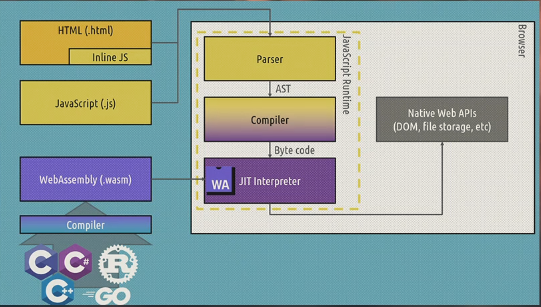
\includegraphics[scale=0.7]{figure/WasmVSJavascript.PNG}}
	\caption{Confronto tra WebAssembly e Javascript}
	\label{fig:WasmVSJavascript}
\end{figure}
Come si pu\'o vedere nella figura 2.3, uno dei motivi per cui WASM \'e pi\'u veloce di Javascript \'e che non deve essere processato e compilato prima di poter essere interpretato, ma solamente scompattato ed eseguito.

La compilazione avviene in modalita AOT(Ahead of Time) e non pi\'u JIT(Just in Time), il che si traduce in un sensibile miglioramenteo delle prestazioni del codice dinamico.
Il C\# quindi non \'e l'unico linguaggio che potr\'a essere utilizzato come partenza per essere compilato in WASM, tuttavia questa tecnologia \'e ci\'o che rende possibile il funzionamento di Blazor.

In questo modello quindi, come visibile dai Chrome Developer Tools, vengono scaricate le DLL dell'applicazione direttamente nel browser dell'utente.

\subsection{Blazor PWA}\label{sez:bpwa}
Lo step successivo per avvicinarsi al client allontanandosi dal modello server \'e poi Blazor PWA.

\'E cos\'i chiamato perch\'e in questo modello Blazor, permette di sviluppare l'interfaccia utente di una Progressive Web App.
Nella figura 2.3 viene riassunto cosa sia una Progressive Web App.

\begin{figure}[H]
	\centerline{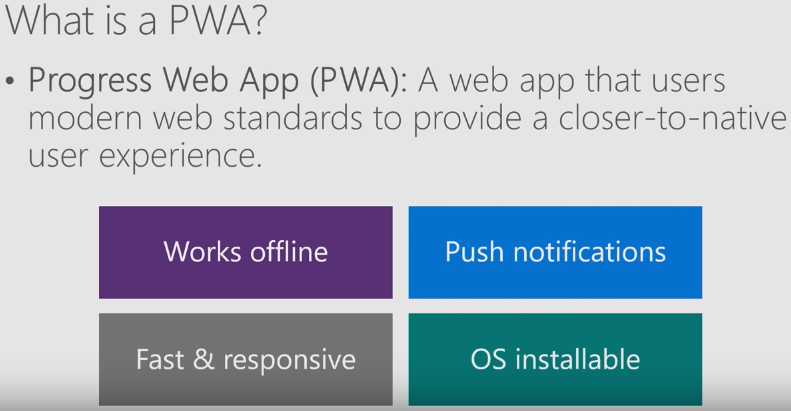
\includegraphics[scale=0.5]{figure/ProgressiveWebApp.png}}
	\caption{Progressive Web Apps}
	\label{fig:WhatIsAPWA}
\end{figure}

In particolare queste sono applicazioni web che hanno la capacit\'a di funzionare anche offline, e che spesso possono essere scaricate in modo persistente sulla macchina dell'utente che le esegue.
Offrono chiaramente una maggiore velocit\'a di esecuzione e la possibilit\'a di sfruttare alcune API native.
Ad esempio possono essere utilizzate quando la necessit\'a \'e quella di utilizzare le notifiche push native del SO che sta utilizzando il client(e.g. Windows).

Per realizzarne una in Blazor al momento, bisogna partire dal modello Blazor WebAssembly aggiungendo un manifesto che descriva le capacit\'a dell'applicazione, i permessi richiesti e l'icona da utilizzare una volta installata, oltre chiaramente a dover implementare l'applicazione in modo che possa lavorare anche offline, basandosi su un service worker.\cite{blazorPWA}
\pagebreak

\section{Modelli in roadmap}
\subsection{Blazor Hybrid}\label{sez:bhybrid}
Questo modello di Blazor ed anche il successivo, servono a sviluppare applicazioni native.
Nel modello Hybrid, l'applicazione sviluppata non \'e quindi pi\'u considerabile una web app ma rimane ibrida perch\'e pur essendo un app nativa, utilizza tecnologie web per effettuare il rendering della user interface.

Esempi di Hybrid Apps possono essere applicazioni mobile native, che hanno accesso alle API esposte ad esempio da Android, ma che utilizzano delle WebViews per la gestione dell'interazione dell'utente con la UI.

Un'altro esempio molto interessante sono le applicazioni che sfruttano Electron, che permette di compilare un'applicazione web in un applicazione desktop cross platform.
Infatti utilizzando Electron si pu\'o creare un'applicazione nativa, con l'interfaccia utente scritta utilizzando blazor, facendo in modo che in fase di esecuzione il processo host sia .NET Core(avendo quindi pieno accesso alle capacit\'a native e ad esempio al file system) pur rimanendo cross platform e potendo quindi eseguire su Windows, Linux e Mac.
Di seguito nell'immagine 2.4 si pu\'o vedere una Web Application compilata nativamente con Electron(con target Windows), e quindi eseguita come applicazione desktop:

\begin{figure}[H]
	\centerline{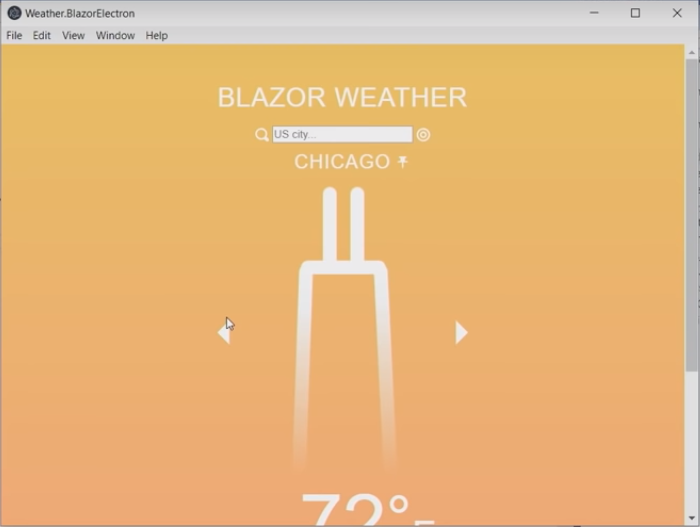
\includegraphics[scale=0.6]{figure/BlazorWeatherElectron.png}}
	\caption{Blazor Hybrid Application}
	\label{fig:BlazorHybridApplication}
\end{figure}

Il codice open source dell'applicazione qui sopra, si trovare al seguente link: https://github.com/danroth27/BlazorWeather/tree/master/BlazorWeather.Electron
\pagebreak



\subsection{Blazor Native}\label{sez:bnative}
Infine esiste il modello Native che \'e possibile grazie al fatto che Blazor \'e stato architettato per poter renderizzare controlli della User Interface che non siano obbligatoriamente strumenti web, e pu\'o quindi integrarsi con controlli nativi.
Il rendering layer \'e infatti intercambiabile, pur essendo quello di default dedicato all'HTML.

Un esempio di applicazione sviluppata utilizzando Blazor per il rendering di controlli nativi nella user interface, si pu\'o vedere durante la presentazione di Steve Sanderson all' evento NDC Oslo di quest'anno, pur non essendo stato ancora rilasciato il codice di un esempio ufficiale.\cite{sandersonNDCBlutter}
In questa applicazione, si \'e scelto di sostituire il default rendering layer per utilizzarne uno custom, utilizzando componenti di Flutter, il toolkit di Google per costruire interfacce utente native CrossPlatform.
Questo modello viene qui citato per completezza, ma al momento non \'e nemmeno presente nella documentazione ufficiale ed \'e solo stato citato da Daniel Roth durante la presentazione dei futuri modelli di Blazor lato client.\cite{blazorNative}

\section{Funzionamento}\label{sez:funzionamento}
Partendo dal codice, come gi\'a anticipato quando si scrive si utilizza un mix di HTML per lo scheletro, CSS per lo stile del documento e C\# preceduto dal relativo carattere di escape(@) per la parte dinamica del codice.
\begin{figure}[H]
	\centerline{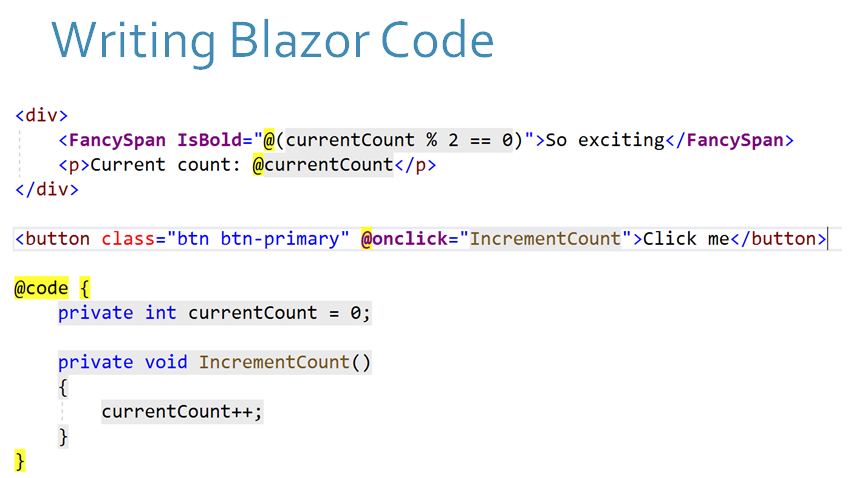
\includegraphics[scale=0.7]{figure/RazorFile.png}}
	\caption{File Razor\cite{ryanNowakNDCSydney}}
	\label{fig:razorFile}
\end{figure}
Si pu\'o scrivere utilizzando questa sintassi solamente nei file che hanno estensione ".razor", il cui esempio si pu\'o trovare in figura 2.7.
Quando l'applicazione viene compilata, i file .razor vengono utilizzati come input per generare dei file C\#(quindi con estensione .cs) equivalenti al codice che si \'e descritto.\cite{ryanNowakNDCSydney}
Un esempio di output di file razor compilato, generato a partire da quello in figura 2.7 \'e visibile in figura 2.8.
\begin{figure}[H]
	\centerline{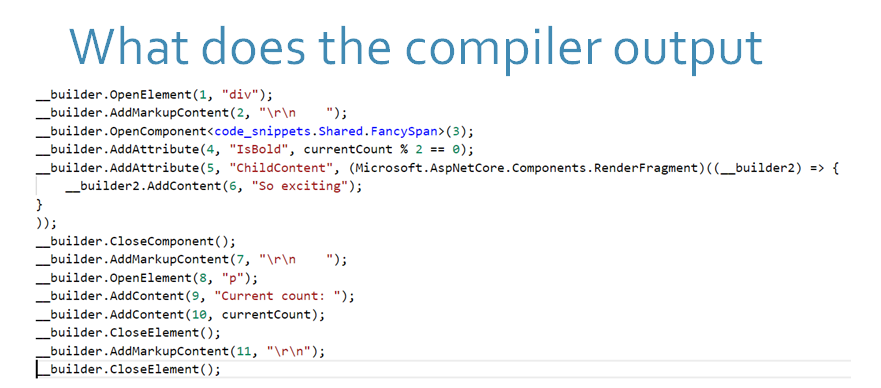
\includegraphics[scale=0.75]{figure/RazorFileCompiled.PNG}}
	\caption{Output\cite{ryanNowakNDCSydney}}
	\label{fig:compiledRazorFile}
\end{figure}

Saranno poi questi file ad essere effettivamente utilizzati da Roslyn(che \'e il nome del compilatore open-source del linguaggio C\#) e a finire nella DLL generata come output dal progetto nel quale si trova il file .razor di partenza.
Questo passaggio non \'e solo necessario per fare in modo che si possano generare le DLL compilate relative ai file di partenza, ma \'e anche il momento in cui viene ottimizzato ci\'o che ha scritto il developer per ogni parte relativa alla UI in ogni file .razor del progetto, riducendolo alle sole primitive di Blazor, che sono vibili nella figura 2.9.

\begin{figure}[H]
	\centerline{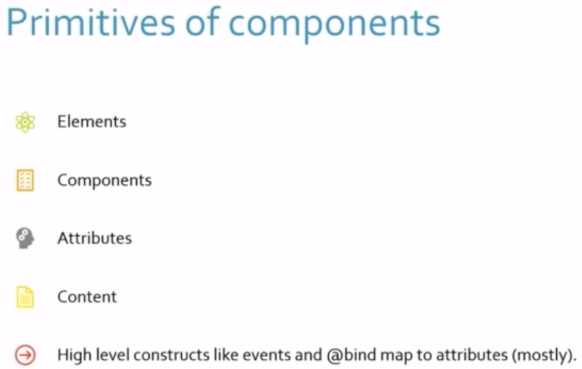
\includegraphics[scale=0.7]{figure/BlazorPrimitives.PNG}}
	\caption{Primitive di Blazor\cite{ryanNowakNDCSydney}}
	\label{fig:BlazorPrimitives}
\end{figure}

In ordine quindi possiamo descrivere le primitive:
\begin{enumerate}
\item Un elemento \'e ad esempio l'elemento html "div";
\item Un component \'e un altro componente(file .razor) che viene utilizzato nel file che si sta compilando;
\item Un attributo \'e appunto un attributo di un elemento html, o un parametro passato in ingresso ad un component;
\item Un contenuto \'e del testo, costante o basato su un parametro, inserito all'interno di un elemento html;
\item L'ultima primitiva di un componente Blazor sono sostanzialmente gli eventi che vengono gestiti dal componente che si sta compilando e le direttive di bind che quindi collegano e mantengono sincronizzate due variabili.
\end{enumerate}

\pagebreak
\chapter{Confronto tra Client e Server}\label{cap:scalprocont}
\section{Scalabilit\`a}\label{sez:scalabilita}
La Scalabilit\`a, ossia la capacit\`a dell'applicazione di resistere all'aumentare del numero di utenti concorrenti che ne usufruiscono, dipende fortemente dal modello scelto, come anche dalla tipologia di applicazione sviluppata.
Quindi scegliere il modello pi\`u adatto non \`e banale e non esiste una soluzione univoca.

Il problemi introdotti dalla scalabilit\`a comunque sono fondamentalmente diversi tra Blazor Server, e tutti gli altri modelli.
Questo principalmente per 3 motivi:
\begin{enumerate}
	\item Blazor Server delega completamente al server che ospita l'applicazione il carico computazionale necessario per gestire ogni singolo evento della UI di ogni sessione per ogni utente connesso, compreso il salvataggio in memoria RAM dello stato di ciascuna UI durante l'utilizzo dell'applicazione.
	Infatti ad ogni browser, per ogni sessione, dopo l'inizializzazione arrivano solamente le minime differenze necessarie per effettuare il render della UI rispetto al frame precedente, ogni volta che deve cambiare qualcosa.
	Ci\`o implica che la potenza del server debba tener conto di eventuali picchi di utenze, e debba avere a disposizione sufficiente RAM per poter mantenere in memoria lo stato dell'applicazione di ciascun utente concorrente connesso.
	
	\item Il secondo \`e che Blazor Server, necessita di almeno una connessione costante ed affidabile con ogni sessione di ogni utente collegato.
	
	\item Il terzo \`e che questo modello sfrutta SignalR, che per funzionare al meglio utilizza il protocollo di trasporto WebSocket, quindi la macchina server sul quale viene ospitata l'applicazione Blazor \`e consigliato che lo supporti, pur non essendo necessario.
\end{enumerate}

Gli altri modelli invece sfruttano l'hardware di ogni client connesso, come solitamente avviene per le SPA odierne.
Sono quindi in linea con il comportamento degli altri framework basati su Javascript come Angular o React, in particolare Blazor WebAssembly. 
Di seguito verranno quindi confrontati pro e contro dell'utilizzo del modello Blazor Server e del modello Blazor WebAssembly, partendo dai punti evidenziati nella figura \ref{fig:blazorModelsProCons}.
\begin{figure}[H]
	\centerline{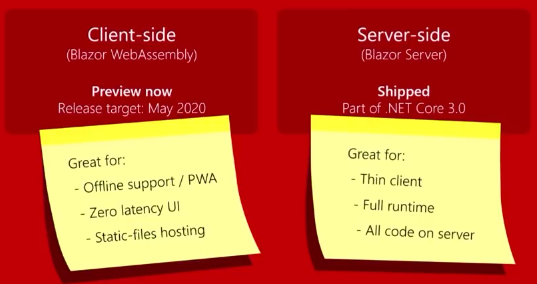
\includegraphics[scale=0.8]{figure/ClientServerProCons.png}}
	\caption{Confronto Modelli Client-Server}
	\label{fig:blazorModelsProCons}
\end{figure}

\section{Blazor Server}\label{sez:scalabilitaBServer}
\subsection{Pro}\label{sez:proBServer}
Blazor Server vanta, come primo punto a favore, il fatto di essere stato creato per essere una soluzione completa, ma che pu\`o essere utilizzata in modo complementare in applicazioni gi\`a esistenti che ad esempio si basano su Razor.
Si pu\`o quindi andare ad ampliare queste applicazioni senza doverle riscrivere da zero.
In questo modo si possono continuare a sfruttare le pagine completamente renderizzate lato server dove necessario, ma si possono anche gestire le interazioni del client con la UI potendo referenziare codice C\# senza doverlo riscrivere in Javascript o anche solo passare tramite JS, in parti dell'applicazione dove si ritiene sia pi\`u adatto farlo.

Un altro grande pro di questo modello \`e il fatto di poter delegare al server la responsabilit\`a di dover sopportare un peso maggiore, al crescere dell'applicazione, mentre il client non deve scaricare pi\`u dati.
Infatti i file scaricati lato client sono solo quelli necessari all'inizializzazione della UI e allo stabilimento di una connessione con il server, che quindi al crescere del peso dell'applicazione, non invia dati in pi\`u ai client, ma continua solamente a inviare le differenze della UI rispetto allo stato precedente.
Questo secondo vantaggio, rende il modello ideale per i casi in cui si deve creare un'applicazione per quale i client che la utilizzeranno potrebbero avere a disposizione computer o cellulari a basso costo.

Il terzo punto a favore, molto utile durante lo sviluppo di applicazioni per le quali la segretezza del codice sorgente risulta critica, \`e che il codice dinamico dell'applicazione sviluppata comprese eventuali logiche di business, non arrivano mai al client che riceve solamente i risultati delle interazioni, in quanto tutto il codice sviluppato viene eseguito(e rimane) lato server dopo la connessione iniziale.

Il quarto punto a favore, \`e che essendo questo modello pronto per produzione, si trovano gi\`a oggi diverse guide online di utenti che hanno provato ad utilizzarlo e che si sono scontrati con i principali problemi esistenti, e in caso di problemi si pu\`o eseguire il debug del codice scritto utilizzando Visual Studio 2019 o Visual Studio Code o ricevere supporto ufficiale da Microsoft nel caso si trovi un problema negli strumenti che si hanno a disposizione.

Infine il fatto che l'applicazione esegua sul server, implica che si possa utilizzare l'intero runtime di .NET Core, che implementa completamente il .NET Standard 2.0.
\subsection{Contro}\label{sez:controBServer}
Il principale punto a sfavore di Blazor Server \`e la gi\`a citata RAM consumata da ogni UI per ogni sessione di ogni utente che utilizza l'applicazione.
Un benchmark eseguito da Microsoft a tal proposito, ha mostrato come il principale collo di bottiglia di un'applicazione Blazor sia proprio la RAM.
Microsoft ha dichiarato che hanno stimato vengano occupati in media 250 KB in RAM per ogni nuova connessione di un utente ad un'applicazione base di tipo "hello world" e consigliano di dedicare almeno 273 KB per utente se non si ha chiaro da dove partire. Durante il test di carico svolto da Microsoft \`e stata utilizzata una sola macchina virtuale Azure di fascia medio-bassa(Standard D1V2)come server per ospitare l'applicazione Blazor, avendo quindi a disposizione 3.5 GB di RAM e le caratteristiche visibili in figura \ref{fig:vmStandardD1V2}.

\begin{figure}[H]
	\centerline{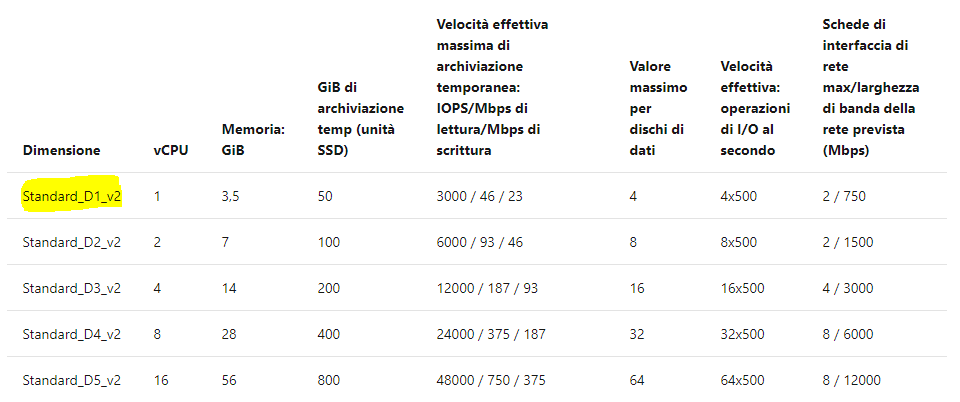
\includegraphics[scale=0.5]{figure/Standard_D1_V2.PNG}}
	\caption{Parametri VM utilizzata per il test di carico}
	\label{fig:vmStandardD1V2}
\end{figure}

Con questi parametri, l'applicazione \`e stata in grado di gestire 5000 utenti concorrenti senza perdita significativa di performance \cite{blazorModelsScenarios} \cite{bServerConcurrentUsersTest}.
Bisogna quindi tener conto che al crescere delle informazioni da tenere in memoria per ciascun utente, l'applicazione sviluppata richieder\`a pi\`u RAM per ciascuno, quindi per questo modello i costi dell'infrastruttura dipendono fortemente dai volumi di utenti concorrenti che la utilizzano.

Un altro punto a sfavore, \`e la certezza che l'applicazione non sar\`a performante per gli utenti che al momento del collegamento si trovano molto lontani(ad esempio in un continente diverso) dal server sulla quale questa \`e ospitata.
Questo avviene perch\`e ogni update della UI deve prima avvenire sul server, quindi la latenza(ping) e la sua variazione(jitter) diventano estremamente importanti per l'esperienza dell'utente.

Infine bisogna tener conto che ogni utente che vuole poter utilizzare l'applicazione, deve potersi connettere ad essa, e restarci connesso per tutta la durata del suo utilizzo, dato che se la connessione SignalR sulla quale si basa Blazor Server per funzionare viene a mancare, in automatico Blazor prover\`a a ricollegarsi al server, ma fino a quando non ci riuscir\`a l'applicazione sar\`a inutilizzabile.

\pagebreak

\section{Blazor WebAssembly}\label{sez:scalabilitaBWA}
\subsection{Pro}\label{sez:proBWA}
Il principale vantaggio di Blazor WebAssembly, specialmente in applicazioni complesse, \`e quello di poter sfruttare le risorse dei client che vogliono utilizzare l'applicazione, senza sovraccaricare il server, specialmente quando il numero di utilizzatori \`e molto alto.
Questo modello infatti, dopo lo scaricamento iniziale dell'applicazione, del runtime dotnet.wasm e delle DLL sulle quali l'applicazione si basa, si pu\`o procedere ed utilizzarla senza pi\`u essere collegati ad internet, almeno per ogni parte nella quale non si cerca di comunicare in modo sincrono con il server.

Altro grande vantaggio, \`e quindi il fatto che dopo lo scaricamento iniziale e l'inizializzazione, l'applicazione sar\`a responsiva senza alcuna latenza, dato che al contrario del modello Blazor Server, la gestione degli eventi da parte dei component di Blazor avviene in locale, senza dover comunicare ogni volta con il server.

Un altro punto a favore al quale prestare attenzione \`e la maggiore facilit\`a con cui si pu\`o trasformare questo modello in una PWA.
In alcuni casi questo modello pu\`o essere la scelta giusta e in futuro un'applicazione di questo tipo potrebbe risultare anche pi\`u veloce di un'applicazione equivalente con componenti scritti in Javascript, dato che il codice dei componenti Blazor per ora viene compilato nel .NET Intermediate Language come visibile nella figura \ref{fig:CLR} e poi interpretato lato client dal runtime Mono tradotto in WebAssembly contenuto nel file dotnet.wasm.

Il fatto stesso di essere equivalente ad un'applicazione moderna scritta usando Javascript agli occhi di un utente ma di poter arrivare ad avere prestazioni migliori e di scrivere in un linguaggio diverso dal solo javascript, rende questo modello estremamente importante e indicato per applicazioni dove ad esempio si vuole poter condividere il codice di validazione ed utilizzarlo tra frontend e backend.
Un'altra categoria di applicazioni per le quali Blazor WebAssembly pu\`o risultare pi\`u indicato, \`e quella dei videogiochi con alta frequenza di aggiornamento nella UI dell'utente, con particolare enfasi su quelli per i quali la grafica \`e complessa e senza interazione multiplayer.
In questi casi risulterebbe inutilmente lento e costoso far avvenire i cambiamenti lato server, poich\`e gli utenti incontrerebbero lag e un'esperienza sicuramente non ideale.
 
\subsection{Contro}\label{sez:controBWA}
Il primo svantaggio di Blazor WebAssembly \`e quindi il peso dell'applicazione, che influisce negativamente sullo scaricamento iniziale.
Ci\`o implica anche che quanto pi\`u codice viene scaricato, tanto pi\`u pu\`o essere studiato e utilizzato per capire logiche di business o cercare modi per attaccare il server.
Questa cosa \`e vera anche per le applicazioni odierne scritte utilizzando Javascript, ma rimane uno svantaggio perch\`e il modello Blazor Server non presenta questa caratteristica.

Un ulteriore svantaggio da tenere in considerazione, \`e che come per ogni nuova tecnologia, la documentazione, il supporto della community, e le librerie dedicate, in questo primo momento sono e saranno fortemente limitate rispetto a framework per UI basati su Javascript equivalenti in teoria ma ben pi\`u consolidati e diffusi in pratica.
Il modello Blazor WebAssembly inoltre, sfruttando il WebAssembly, necessita che il browser di ogni client che vuole poter utilizzare l'applicazione lo supporti.

L'ultima grande pecca di questo modello \`e sicuramente il fatto che sia ancora immaturo.
Questo principalmente perch\`e gli strumenti a disposizione sono ancora relativamente acerbi e anche se dal rilascio ufficiale \`e possibile eseguire in debug e impostare dei breaking points direttamente in visual studio sia per il codice JS, sia per il codice C\# lato client che per il codice C\# lato server, non \`e presente l'hot reload.
Ci\`o rende quindi tediosa la modifica di ogni file durante l'esecuzione, dato che per poter vedere il risultato delle modifiche effettuate \`e poi necessario ricompilare e rilanciare l'applicazione.
In secondo luogo perch\`e pur essendo Blazor WebAssembly ottimizzato per essere molto efficiente durante il rendering della UI, c'\`e ancora molto margine di miglioramento, specialmente quando l'applicazione Blazor scritta \`e CPU intensive.
Questo semplicemente perch\`e ora come ora il codice viene scaricato sotto forma di DLL ed interpretato dal runtime di Mono tradotto in WASM, e non direttamente eseguito.
D. Roth ha dichiarato che il team che si occupa di sviluppare Blazor sta lavorando per rendere possibile la compilazione del codice da .NET direttamente in WASM, cos\`i da ottenere performance decisamente migliori\cite{blazorModelsScenarios}.

\section{BlazorPong a confronto}\label{sez:scalabilitaBWA}
Il miglior modello, per questa tipologia di applicazione, \`e Blazor Server, ammesso che si abbiano a disposizione le risorse per poterlo supportare(in questo caso le risorse sono scarse e per questo gratuite seppur sufficienti per le necessit\`a delle applicazioni sviluppate per questo lavoro di tesi).
Questo \`e visibile specialmente in termini di prestazioni dei due progetti le cui demo sono disponibili nel repository github BlazorPong.

Principalmente possiamo ridurre il vantaggio di Blazor Server a:
\begin{enumerate}
	\item Un avvio molto pi\`u rapido e una giocabilit\`a migliore, ideali per il raggiungimento di un pubblico pi\`u vasto vista la possibilit\`a di giocare anche con apparecchi meno potenti di quelli necessari per eseguire la computazione del codice lato Client;
	\item In Blazor WASM il codice per poi poter effettuare il render della UI(e quindi i component) viene scaricato durante il primo download dell'applicazione, che risulta quindi anche se solo la prima volta, estremamente pi\`u lento se ci si trova con una velocit\`a di connessione limitata;
\end{enumerate}

In particolare la quantit\`a di dati scaricati al primo avvio di BlazorPong Server \`e meno di 200 kilobyte come visibile nella figura \ref{fig:blazorpongServerWeigth}.

\begin{figure}[H]
	\centerline{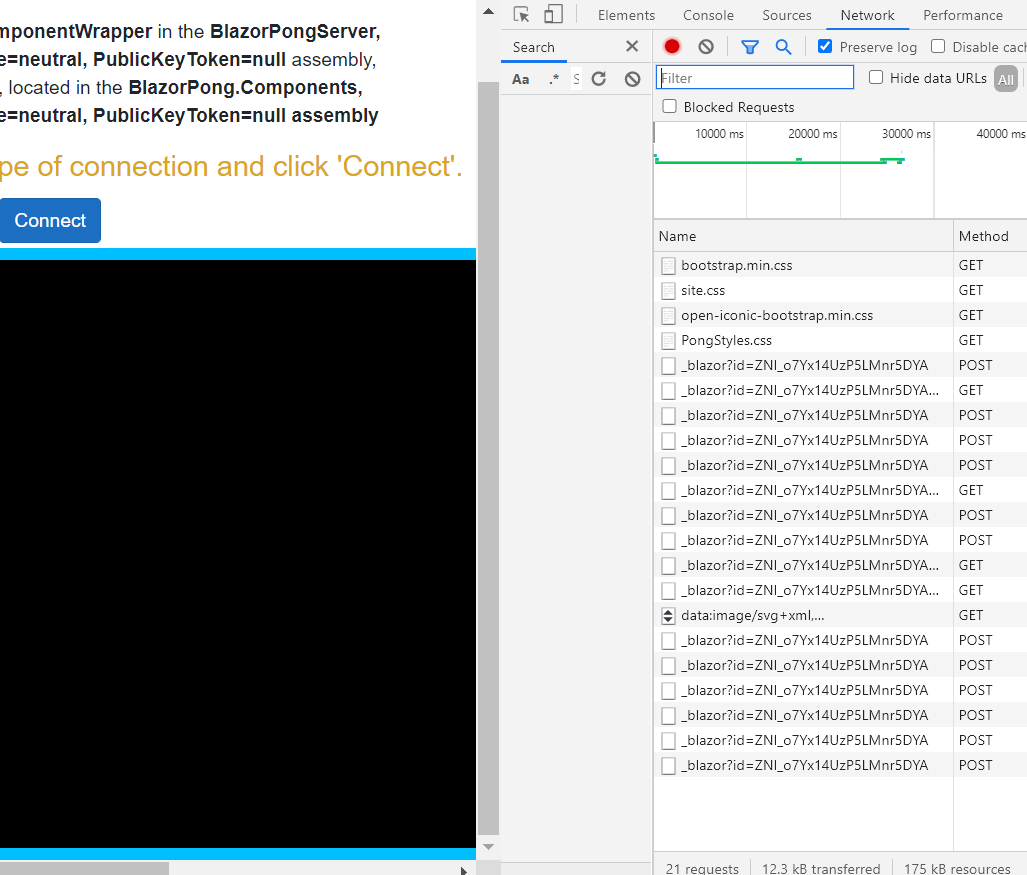
\includegraphics[scale=0.5]{figure/blazorpongServerWeigth.PNG}}
	\caption{Peso primo avvio blazorpong server.}
	\label{fig:blazorpongServerWeigth}
\end{figure}

Il peso dell'applicazione versione WASM \`e invece circa 20 megabyte come visibile in figura \ref{fig:blazorpongClientWeigth}.

\begin{figure}[H]
	\centerline{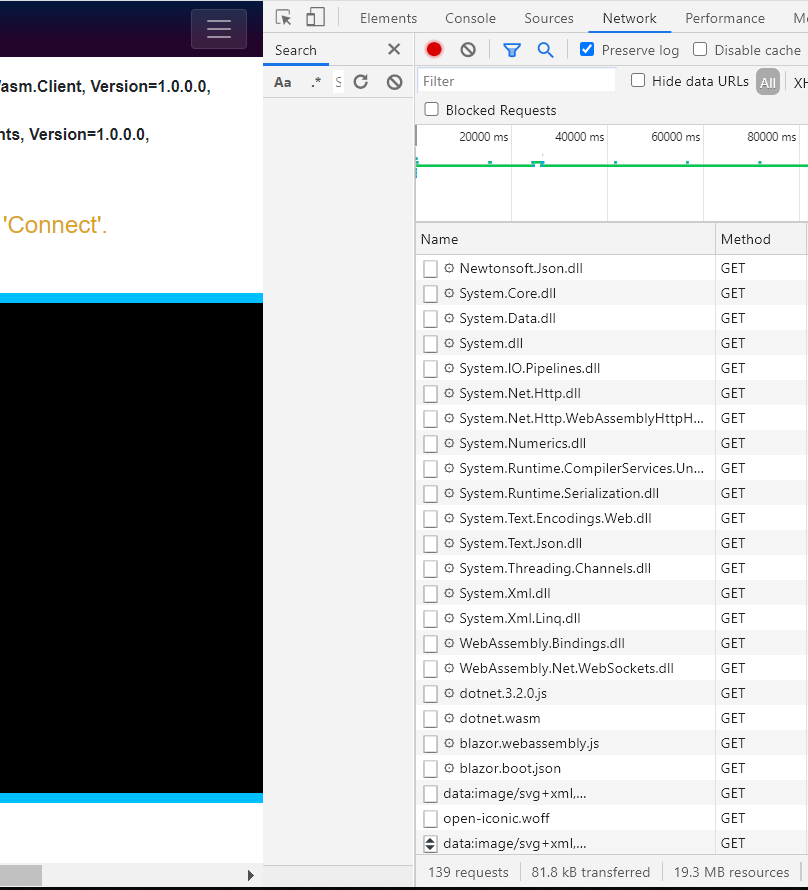
\includegraphics[scale=0.5]{figure/blazorpongClientWeigth.PNG}}
	\caption{Peso primo avvio blazorpong client.}
	\label{fig:blazorpongClientWeigth}
\end{figure}
\chapter{Conclusioni}\label{cap:conclusioni}
\section{Conclusioni}\label{sez:conclusioni}
\section{Futuro del progetto}\label{sez:futuro}
\begin{figure}[H]
	\centerline{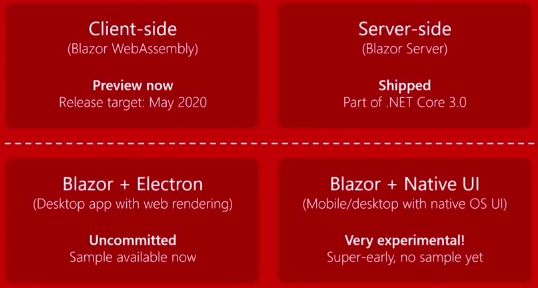
\includegraphics[scale=0.8]{figure/ModelsSupportedOrNot.png}}
	\caption{Modelli blazor e supporto}
	\label{fig:supportedBlazorModels}
\end{figure}

Onbeforeunload
\include{sorgenti/cap_5}

\appendix
%\chapter{Prova}\label{cap:prova}

\section{Pippo}\label{sez:pippo}

A seguito della crescente diffusione ...

%alcuni risultati sul risparmio
\section{Ciu Ciu}\label{sec:ciu_ciu}

Prima di analizzare nel dettaglio ...

\begin{thebibliography}{999}

\bibitem{Hoff}
M.~Wanyoike,
Disponibile: https://blog.logrocket.com/history-of-frontend-frameworks.

\bibitem{jquery}
Disponibile: https://en.wikipedia.org/wiki/JQuery.

\bibitem{razor}
Disponibile: https://docs.microsoft.com/en-us/aspnet/core/razor-pages/?view=aspnetcore-3.0\&tabs=visual-studio.

%
%\bibitem{MathewsSicuranza}
%V.~J.~Mathews e G.~L.~Sicuranza,
%{\em Polynomial Signal Processing},
%New York: Wiley, 2000, pp.100-120.
%
%\bibitem{CariniMumoloSicuranza}
%A.~Carini, E.~Mumolo e G. L.~Sicuranza,
%``V-Vector Algebra and Volterra Filters'',
%in {\em Advances in Imaging \& Electron Physics}, Vol.~124,
%P.~W.~Hawkes, Ed., San Diego: Academic Press, 2003, pp.~1-61. 
%
%\bibitem{Carini}
%A.~Carini,
%``Efficient NLMS and RLS Algorithms for Perfect and Imperfect Periodic Sequences'',
%{\em IEEE Transactions on Signal Processing}, vol.~58, No.~4, pp.~2048-2059, Aprile 2010.
%
%\bibitem{CariniMathewsSicuranza}
%A.~Carini, V.~J.~Mathews e G.~L.~Sicuranza,
%``Efficient NLMS and RLS Algorithms for a Class of Nonlinear Filters Using Periodic Input Sequences'',
%{\em Proceedings of 36th International Conference on Acoustics, Speech, and Signal Processing, ICASSP 2011},
%Prague, Czech Republic, Maggio 22-27, 2011, pp.~4280-4283.
%
%\bibitem{CariniBrv}
%A.~Carini,
%``Filter for the Equalization and/or Linearization of Nonlinear Systems'',
%Brevetto Europeo EP~0939487A2, 25 Febbraio~1999.
%
%\bibitem{Standard}
%{\em IEEE Criteria for Class IE Electric Systems}, IEEE Standard 308, 1969.
%
%\bibitem{Jones}
%J.~Jones,
%{\em Networks} (2nd ed.) [Online] (10 Maggio 1991). [Ultimo accesso: 11 Maggio 2001].
%Disponibile: http://www.atm.com 

%\bibitem{Vidmar}
%R.~J.~Vidmar,
%{\em On the Use of Atmospheric Plasmas as Electromagnetic Reflectors} [Online]. (1994).
%[Ultimo accesso: 11 Maggio 2001]
%Disponibile FTP: atmnext.usc.edu Directory: pub/etext/1994 File: atmosplasma.txt

%\bibitem{Biglieri-84}
%E.~Biglieri, A.~Gersho, R.~D.~Gitlin and T.~L.~Lim, ``Adaptive Cancellation of Nonlinear Intersymbol
%Interference for Voiceband Data Transmission'', {\em IEEE Journal on Selected Areas in Communications},
%Vol.~SAC-2, No.~5, Sep.~1984, pp.~765-777.
%
%\bibitem{Biglieri-88}
%E.~Biglieri, S.~Barberis and M.~Catena, ``Analysis and Compensation of Nonlinearities in Digital
%Transmission Systems'', {\em IEEE Journal on Selected Areas in Communications}, Vol.~6, No.~1, Jan.~1988,
%pp.~42-51.
%
%\bibitem{Biglieri-89}
%E.~Biglieri, M.~Elia and L.~Lopresti, ``The Optimal Linear Receiving Filter for Digital Transmission Over
%Nonlinear Channels'', {\em IEEE Trans. on Information Theory}, Vol.~35, No.~3, May 1989, pp.~620-625.
%
%\bibitem{Biglieri-94}
%E.~Biglieri, E.~Chiaberto, G.P.~Maccone and E.~Viterbo, ``Compensation of Nonlinearities in High-Density
%Magnetic Recording Channels'', {\em IEEE Trans. on Magnetics}, Vol.~30, No.~6, Nov.~1994, pp.~5079-5086.
%
%\bibitem{bitmead-80}
%R.R.~Bitmead and B.D.O.~Anderson, ``Lyapunov Techniques for the Exponential Stability of Linear Difference
%Equations with Random Coefficients'', {\em IEEE Trans. on Automatic Control,} Vol.~AC-25, No.~4, Aug. 1980,
%pp.782-787.
%
%\bibitem{Bose-95}
%T.~Bose and D.A.~Trautman, ``Stability of the Quantized LMS Algorithm'', {\em Circuits Systems Signal
%Processing}, Vol.~14, No.~5, 1995, pp.~587-602.
%
%\bibitem{Bose-951}
%T.~Bose and M.~Q.~Chen, ``BIBO Stability of the Discrete Bilinear Systems'', {\em Digital Signal Processing:
%A Review Journal}, Vol.~5, No.~3, July 1995, pp.~160-166.
%
%\bibitem{Carini-95}
%A.~Carini and E.~Mumolo, ``A Novel Algebraic Formulation for the Development of Adaptive Volterra Filtering
%Algorithms'', {\em Proceedings of 1995 IEEE Workshop on Nonlinear Signal and Image Processing}, June 20-22
%1995, Neos Marmaras, Halkidiki, Greece, pp.~943-946.
%
%\bibitem{Carini-951}
%A.~Carini and E.~Mumolo, ``Adaptive Stabilization of Recursive Second Order Polynomial Filters by Means of a
%Stability Test'', {\em Proceedings of 1995 IEEE Workshop on Nonlinear Signal and Image Processing}, June
%20-22 1995, Neos Marmaras, Halkidiki, Greece, pp.~939-942.
%
%\bibitem{Carini-96}
%A.~Carini, ``A Novel Givens Rotation Based Fast SQR-RLS Algorithm'', {\em Proc. of EUSIPCO-96, VIII European
%Signal Processing Conference}, Trieste, Italy, September 10-13 1996, pp.~1235-1238.
%
%\bibitem{Carini-97}
%A.~Carini and E.~Mumolo, ``Fast Square-Root RLS Adaptive Filtering Algorithms'', {\em Signal Processing},
%Vol.~57, No.~3, Mar.~1997, pp.~233-250.
%
%\bibitem{Carini-971}
%A.~Carini, G.L.~Sicuranza and V.J.~Mathews, ``On the Inversion of Certain Nonlinear Systems'', {\em IEEE
%Signal Processing Letters}, Dec.~1997.

\end{thebibliography}


\ringraziamenti
Vorrei ringraziare il professor Lattanzi per avermi aiutato a scrivere questa tesi, i miei genitori per avermi permesso di procedere facendo di testa mia su un percorso a loro estraneo, e la mia ragazza Ivana per aver creduto in me e nelle mie capacit� anche quando non l'ho fatto io.

\end{document}
